\chapter{Path Planning Algorithms}
\section{Overview}

The output of the path generator should be a single trajectory that completely connects and covers all elements of the drawing.

Derived from the requirements, three different elements were identified as part of drawing (illustrated in \autoref{fig:elements_def}):

\begin{description}
\item[Polyline] A line consisting of $2$ to $n$ vertices.
\item[Polygon] A closed line, consisting of $2$ to $n$ vertices, where the last segment is a closing one. Vertex $v_{n+1}$ coincides with $v_0$.
\item[Filled Polygon] Defined in the same way as the polygon, except that the inner space should be filled by a generated trajectory. Another difference is that the filled polygon can also contain holes, which should not be covered and are excluded from the fill trajectory.
\end{description}

The path generation happens in three steps: First, the polygons that have to be filled are selected and the fill algorithm is seperately executed for each of the polygons with polygon specific settings. In a second step all of the drawing elements are connected by an open tour and a Traveling Salesman heuristic minimizes the total driving distance. As last step, the connections are shaped with curves that conform to  a curvature limit.

Each of those steps will be discussed in detail in this section.

\begin{figure}
\centering
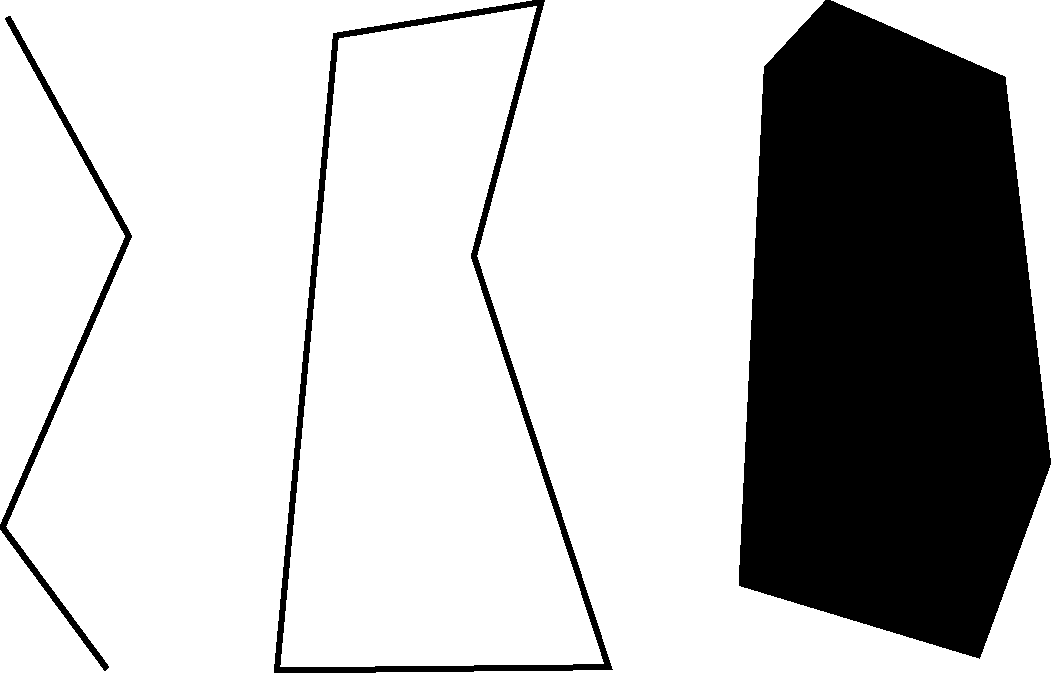
\includegraphics[width=0.6\textwidth]{images/path_planning/line_polygon_definition.pdf}
\caption{Polyline, polygon and filled polygon}
\label{fig:elements_def}
\end{figure}

% you discuss the lines, closed lines, filled polygons
% then you explain the structure that you work on elements separately and the connect them with TSP.
\section{Polygon Filling}

\subsection{Related Work}

Over time several complete coverage algorithms have been developed, and some distinctions can be made. 

One category of solutions for the surface coverage  was developed for robots that do not know the surroundings beforehand and use a variant of \textit{simultaneous localization and mapping} (SLAM) to gather knowledge of the environment. 

Coverage algorithms exist for household applications like autonomous vacuum cleaners or autonomous lawn mowers but also search and rescue robots usually and they  do not care if they visit the same spot twice. The target for those algorithms is rather to achieve complete coverage of an previously unknown terrain in sensible time. Usually, the complete surface coverage algorithms in are also connected with online map generation techniques \textit{SLAM}, whereas the path generation for the BeachBot should happen offline.

However, in agricultural applications some interesting algorithms have been found, which served as inspiration for the explorations presented in this thesis. Especially \citep{ROB:ROB20300}, who hinted at exploiting the straight skeleton algorithm to generate the inset polygons. An optimization strategy is employed to find the shortest trajectory through the field by repeatedly offsetting the remainding shape and traversing all possible ways off filling the shape. The algorithm is relatively computationally intensive, what might be justified when using large agricultural machines but what was not necessary for the goals of this thesis as the benefit of this optimization would be relatively small.

Another field where trajectories have to be generated is in \textit{Computer Aided Machining} (CAM). The process of removing layers of material from a block of metal is quite similar (though inverse, usually) to what is achieved in this thesis. Many publications deal with the problem of multi-axis milling machines which are far more complex and are also able to move over the machined surface without problem because the machining head can be lifted -- something that is not possible with an autonomous ground vehicle.

One interesting publication in the CAM field is \cite{kao1998optimal} that presents a method to reduce gaps that are present when simply offsetting a polygon with spirals. The presented method could be a possible future improvement to the spiral fill algorithm of \autoref{sec:spiral_fill}.

The OpenCAM library has also been inspected...

\subsection{Mathematical Discussion of Polygons}

The following is a mathematical definition of a polygon (taken from \cite{coxeter1967geometry}):

\enquote{A polygon may be defined as consisting of a number of points (called vertices) and an equal number of line segments (called sides), namely a cyclically ordered set of points in a plane, with no three successive points collinear, together with the line segments joining consecutive pairs of the points. In other words, a polygon is closed broken line lying in a plane}.

Polygons can have several properties that simplify or complicate their treatment:

\begin{description}
\item[Simple] A simple polygon is not self intersecting and has a well-defined interior and exterior.\cite{weisstein_simple_p}
\item[Convex] In the convex case any line can intersect the polygon only at two points. The interior all have to be smaller than 180°.\cite{weisstein_convex_p}
\item[Concave] A concave polygon can be intersected more than twice by a given line. Therefore, at least one interior angle has to be larger than 180°.\cite{weisstein_concave_p}
\item[Self-intersecting] A self intersecting polygon has at least one side which intersects with another side.
\item[Polygon with Holes] A hole of a polygon is an enclosed or partially enclosed area that is not part of the filled surface of the outer polygon.
\end{description}

\begin{figure}
\centering
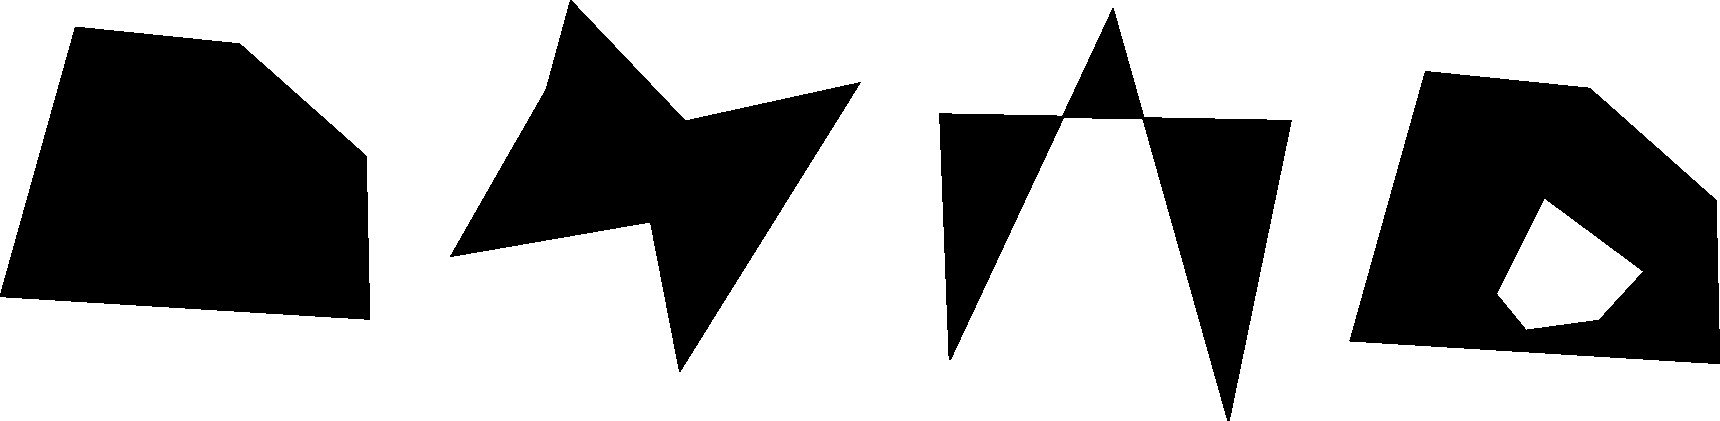
\includegraphics[width=\textwidth]{images/path_planning/polygon_types.pdf}
\caption{Four different polygon types, from left to right: (a) simple and convex, (b) simple and concave, (c) self-intersecting, (d) polygon with a hole}
\label{straight_skel}
\end{figure}

\subsection{Spiral Filling}

The first method to cover the area of an arbitrary polygon is the spiral fill method using inset polygons that are created using the straight skeleton of the polygon.

\subsubsection{Straight Skeleton}

For this thesis, the most interesting property of the straight skeleton is the ability to easily obtain inset polygons with an arbitrary offset. The straight skeleton is defined as the topolgical skeleton of a polygon that is created by moving the edges parallel to themselves inwards at a constant speed and observing the intersections of the vertices (first described by Aichholzer et al. (1995) \cite{Aichholzer:jucs_1_12:a_novel_type_of}). 
It is similar to the median axis of a polygon, but unlike the median axis it is not defined to have a constant distance to the polygon edges. 
Another commonly used offset mechanism for polygons in motion planning is the Minkowski sum. However, there is no defined Minkowski subtraction, which makes the creation of inset polygons more complicated\footnote{It is possible to create an enclosing polygon, subtract the original polygon and offset the enclosing polygon with hole by taking the Minkowski sum (which also offsets the \enquote{hole}).}. An efficient implementation to compute the straight skeleton is discussed by Huber \cite{huber2010computing}.

To create a spiral trajectory, two events that occur during the creation of the straight skeleton have to be kept in mind (see \autoref{straight_skel}): 

\begin{description}
\item[Edge Event] Depending on the length difference between the edges, one edge might be reduced to zero sooner than the others, resulting in an edge event. The neighboring edges are adjacent after the event. At this point, the inset polygon will be reduced by one vertex.
\item[Split Event] A concave polygon will, at some point during the shrinking process, intersect itself. At the intersection point, a split event happens. After the split event, the number of inset polygons is increased by one.
\end{description}

\begin{figure}
\centering
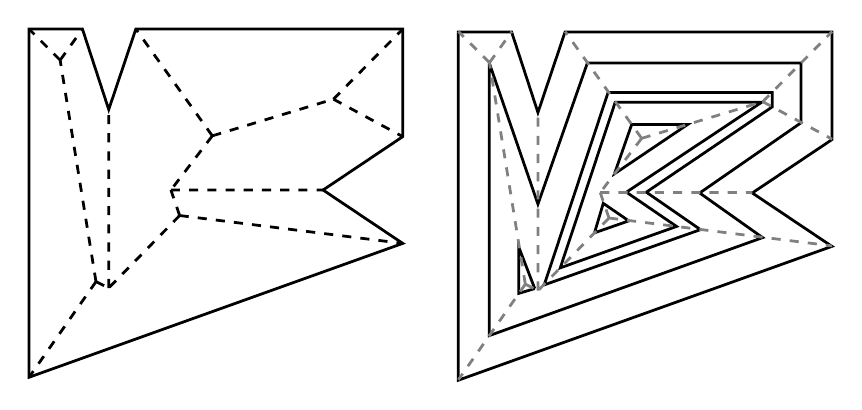
\begin{tikzpicture}[y=0.80pt,x=0.80pt,yscale=-1, inner sep=0pt, outer sep=0pt]
  \path[draw=black,dash pattern=on 3.29pt,line join=miter,line cap=butt,miter
    limit=10.00,line width=1pt] (203.1137,220.5582) --
    (189.0787,206.5192)(203.1137,220.5582) --
    (213.1929,206.5192)(225.0684,323.4860) --
    (225.0684,242.8722)(219.3083,320.6079) --
    (189.0787,363.7948)(219.3083,320.6079) --
    (225.0684,323.4860)(219.3083,320.6079) --
    (203.1137,220.5582)(326.5591,238.1899) --
    (357.8705,255.1070)(326.5591,238.1899) --
    (357.8705,206.5192)(253.1386,279.2212) --
    (321.8807,279.2212)(257.0984,290.7375) --
    (357.8705,303.3315)(257.0984,290.7375) --
    (253.1386,279.2212)(257.0984,290.7375) --
    (225.0684,323.4860)(271.8559,254.7477) --
    (326.5591,238.1899)(271.8559,254.7477) --
    (237.3032,206.5192)(271.8559,254.7477) -- (253.1386,279.2212);
  \path[draw=black,line join=miter,line cap=butt,miter limit=10.00,line
    width=1pt] (189.0787,206.5192) -- (189.0787,363.7948) --
    (357.8705,303.3315) -- (321.8807,279.2212) -- (357.8705,255.1070) --
    (357.8705,206.5192) -- (237.3032,206.5192) -- (225.0684,242.8722) --
    (213.1929,206.5192) -- cycle;
  \path[draw=black,line join=miter,line cap=butt,miter limit=10.00,line
    width=1pt] (382.9398,207.8565) -- (382.9398,365.1321) --
    (551.7316,304.6688) -- (515.7419,280.5585) -- (551.7316,256.4443) --
    (551.7316,207.8565) -- (431.1683,207.8565) -- (418.9296,244.2055) --
    (407.0541,207.8565) -- cycle;
  \path[draw=black,line join=miter,line cap=butt,miter limit=10.00,line
    width=1pt] (382.9398,207.8565);
  \path[draw=black,line join=miter,line cap=butt,miter limit=10.00,line
    width=1pt] (520.4203,239.5272) -- (453.8415,239.5272) --
    (429.0088,314.3887) -- (481.5524,295.6714) -- (458.8792,280.1953) --
    (520.0610,239.5272)(421.0891,322.3044) -- (492.3501,297.1124) --
    (467.8766,280.1953) -- (524.7393,241.6867) -- (524.7393,235.2081) --
    (450.6003,235.2081) -- (421.8077,321.9452)(417.4886,323.7454) --
    (410.2914,305.0281) -- (410.2914,325.9050) --
    (417.4886,323.7454)(444.4809,298.5534) -- (459.9570,293.1526) --
    (448.4407,285.2369) -- (444.4809,298.5534)(461.3980,249.6063) --
    (486.5900,249.6063) -- (453.4783,271.9203) --
    (461.3980,249.2471)(396.9749,221.5323) -- (396.9749,344.9777) --
    (520.4203,300.7129) -- (491.9908,280.5585) -- (537.6966,248.8839) --
    (537.6966,221.8916) -- (441.2436,221.8916) -- (418.9296,285.5961) --
    (396.9749,221.8916);
  \path[draw=gray,dash pattern=on 3.29pt,line join=miter,line cap=butt,miter
    limit=10.00,line width=1pt] (397.0360,221.6940) --
    (383.0010,207.6550)(397.0360,221.6940) --
    (407.1152,207.6550)(418.9907,324.6218) --
    (418.9907,244.0080)(413.2306,321.7437) --
    (383.0010,364.9306)(413.2306,321.7437) --
    (418.9907,324.6218)(413.2306,321.7437) --
    (397.0360,221.6940)(520.4814,239.3257) --
    (551.7928,256.2428)(520.4814,239.3257) --
    (551.7928,207.6550)(447.0609,280.3570) --
    (515.8030,280.3570)(451.0207,291.8733) --
    (551.7928,304.4674)(451.0207,291.8733) --
    (447.0609,280.3570)(451.0207,291.8733) --
    (418.9907,324.6218)(465.7782,255.8835) --
    (520.4814,239.3257)(465.7782,255.8835) --
    (431.2255,207.6550)(465.7782,255.8835) -- (447.0609,280.3570);

\end{tikzpicture}
\caption{Straight skeleton and generated inset polygons (right). Split and edge events are well visible. Figure modified from \cite{Aichholzer:jucs_1_12:a_novel_type_of}.}
\end{figure}


The inset polygons are used to create a spiral fill for the polygons. The procedure is as follows:

\begin{enumerate}
\item The straight skeleton is generated.
\item The first inset polygon is created. The inset distance is the constant width of the rake divided by the number of vertices of the polygon. Through dividing the inset length by the number of vertices in the polygon, one revolution of the spiral will travel one rake distance inwards.
\item If a split event has happened, then it is decided which polygon should be used to extend the current spiral (that is the one with the closer point to the current position). All other newly created polygons are recursively filled by the same algorithm. %Additionally, a starting point to the spiral is passed, so that the beginning of the next spiral will be close to the current one. (The procedure restarts with each split polygon as input at (0)).
\item The closest point to the current point on the inset polygon is searched ($v_n$). The next vertex of the inset polygon in clockwise direction ($v_{n+1}$) is appended to the current spiral
\item The next inset polygon is generated with inset length divided by the number of vertices of the previous inset polygon, and the process continues at (4).

\end{enumerate}

\begin{algorithm}[H]
\begin{algorithmic}
\caption{Spiral Filling}\label{spiral_fill}

\Function{createSpiralFill}{Polygon p, Point startPoint}
\State $RakeWidth \gets \text{(const. rake width for BeachBot)}$
\State $result \gets \text{empty list of points}$
\State $ss \gets \text{getStraightSkeleton}(p)$
\State $lOffset = RakeWidth/p.numVertices()$
\If{$startPoint$} $currPoint \gets startPoint$ 
\Else ~$ currPoint \gets p.firstVertex$ 
\EndIf
\State $insetPolys \gets getOffsetPolygons(ss, lOffset)$`
\While{$insetPolys.numPolys() \geq 1$}
\If{$insetPolys.numPolys() > 1$}
	\State $closestPoly = searchClosestPolygon(insetPolys, currPoint)$
	\ForAll{$\lbrace poly \in insetPolys | poly \not\in closestPoly\rbrace$}
		\State $createSpiralFill(poly, currPoint)$
	\EndFor
	\State $ss \gets getStraightSkeleton(closestPoly)$
	\State $lOffset = RakeWidth/closestPoly.size()$
	\State $insetPolys \gets getOffsetPolygons(ss, lOffset)$
\EndIf
\State $index \gets findClosestIndex(currPoint, insetPolys.firstPoly)$
\State $currPoint \gets insetPolys.firstPoly.pointFromIndex(index + 1)$
\State $result.appendToList(currPoint)$
\State $insetPolys \gets getOffsetPolygons(ss, lOffset)$
\EndWhile
\EndFunction

\end{algorithmic}

\end{algorithm}

The algorithm is both displayed in Algorithm 1 and graphically in \autoref{fig:insetting}. The result of the algorithm is presented in \autoref{fig:gen_spiral}.

\begin{figure}[htbp]
	\centering
    \begin{subfigure}[b]{0.45\textwidth}
    		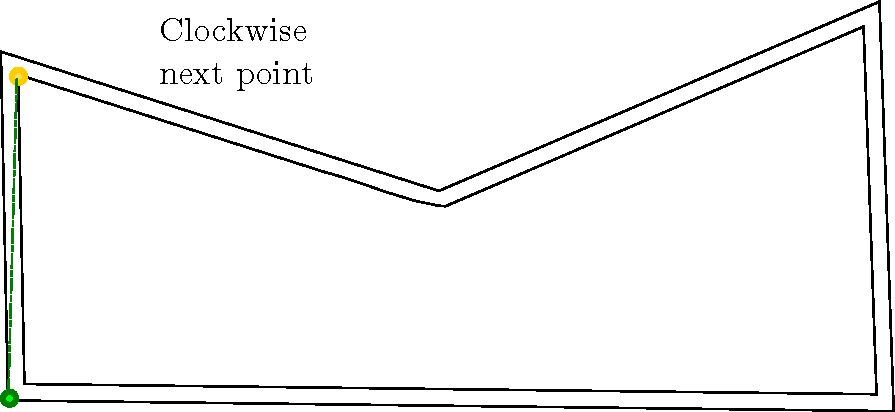
\includegraphics[width=\textwidth]{images/algorithms/spiral_fill/2.pdf}
		\caption{The first inset polygon and the first part of the spiral line}
    \end{subfigure}
    ~
    \begin{subfigure}[b]{0.45\textwidth}
    		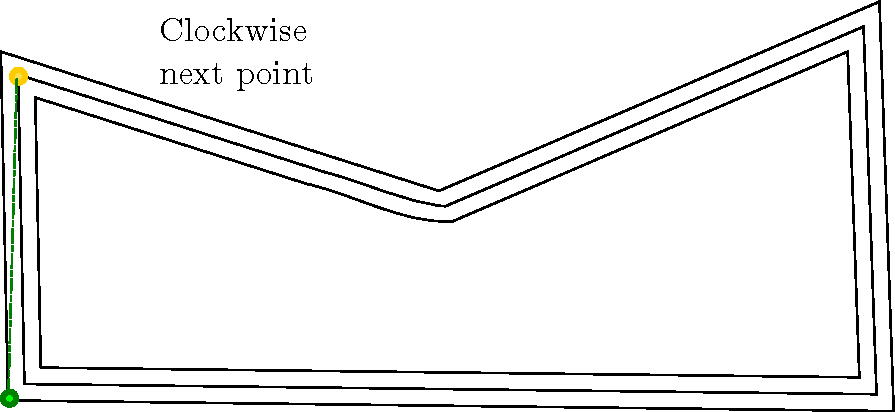
\includegraphics[width=\textwidth]{images/algorithms/spiral_fill/3.pdf}
    		\caption{Next inset polygon generated}
    \end{subfigure}\\
    \begin{subfigure}[b]{0.45\textwidth}
    		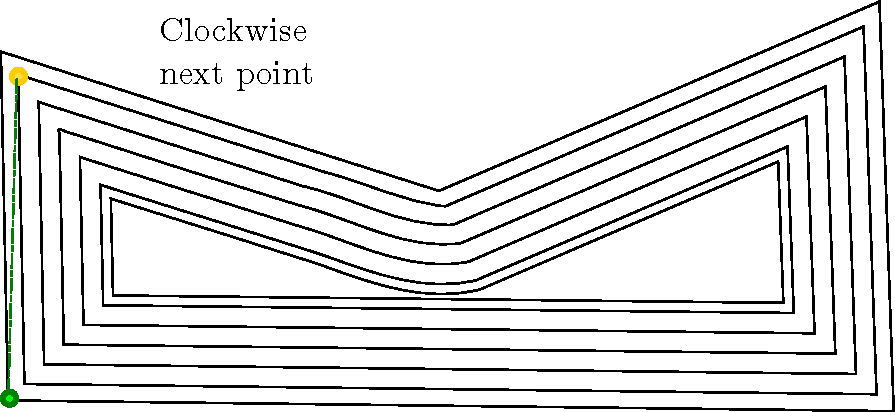
\includegraphics[width=\textwidth]{images/algorithms/spiral_fill/4.pdf}
    		\caption{The polygon right before the \textit{split} happens}
    \end{subfigure}~
    \begin{subfigure}[b]{0.45\textwidth}
    		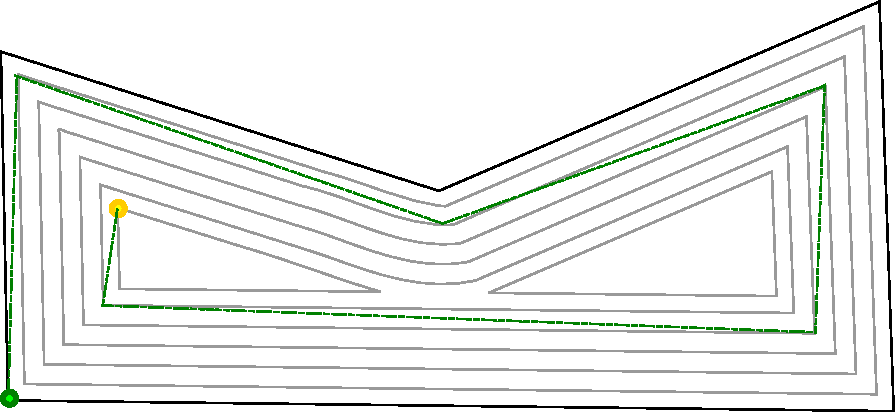
\includegraphics[width=\textwidth]{images/algorithms/spiral_fill/done.pdf}
    		\caption{After split, next polygon was found for continuing the current spiral}

    \end{subfigure}
        \begin{subfigure}[b]{0.45\textwidth}
    		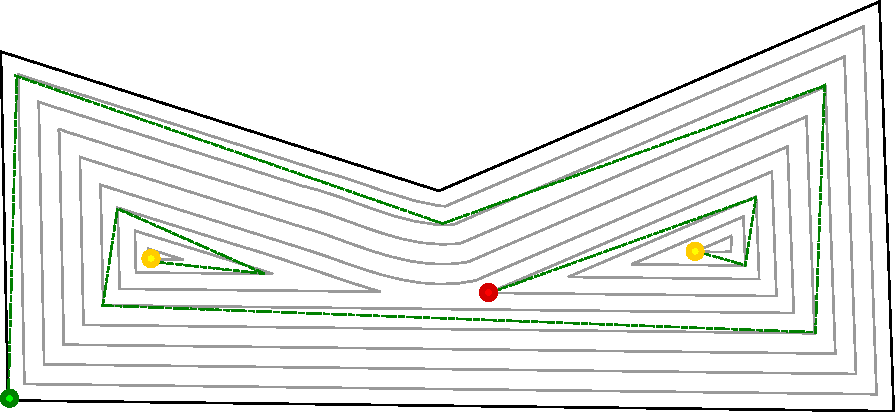
\includegraphics[width=\textwidth]{images/algorithms/spiral_fill/after_done_2.pdf}
    		\caption{Continuing spiral 1 and starting the second spiral. Note how the start point of the second spiral is the closest point to the endpoint of the first.} \label{splitevent}
    \end{subfigure}
\\
        \begin{subfigure}[b]{0.45\textwidth}
    		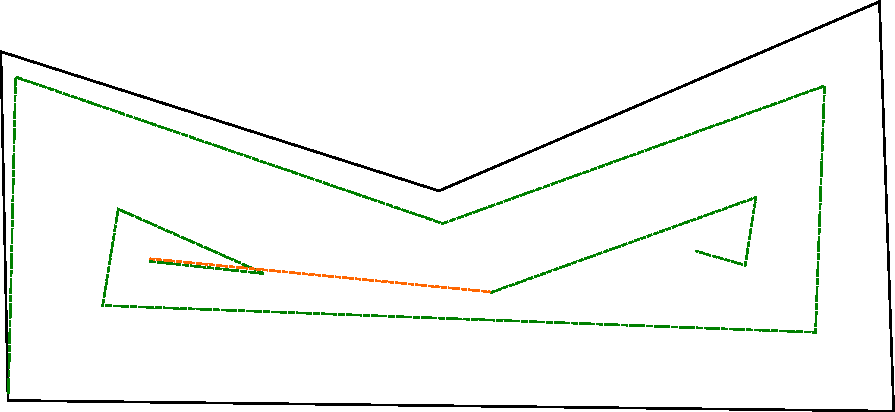
\includegraphics[width=\textwidth]{images/algorithms/spiral_fill/complete_done.pdf}
    		\caption{The completed spiral with all inset polygons removed.}
    \end{subfigure}
	\caption{Generating the fill spiral. Note that this is only an example for illustration purposes. The density of inset polygons for a real application is much higher.} \label{fig:insetting}
\end{figure}

\begin{figure}
\centering
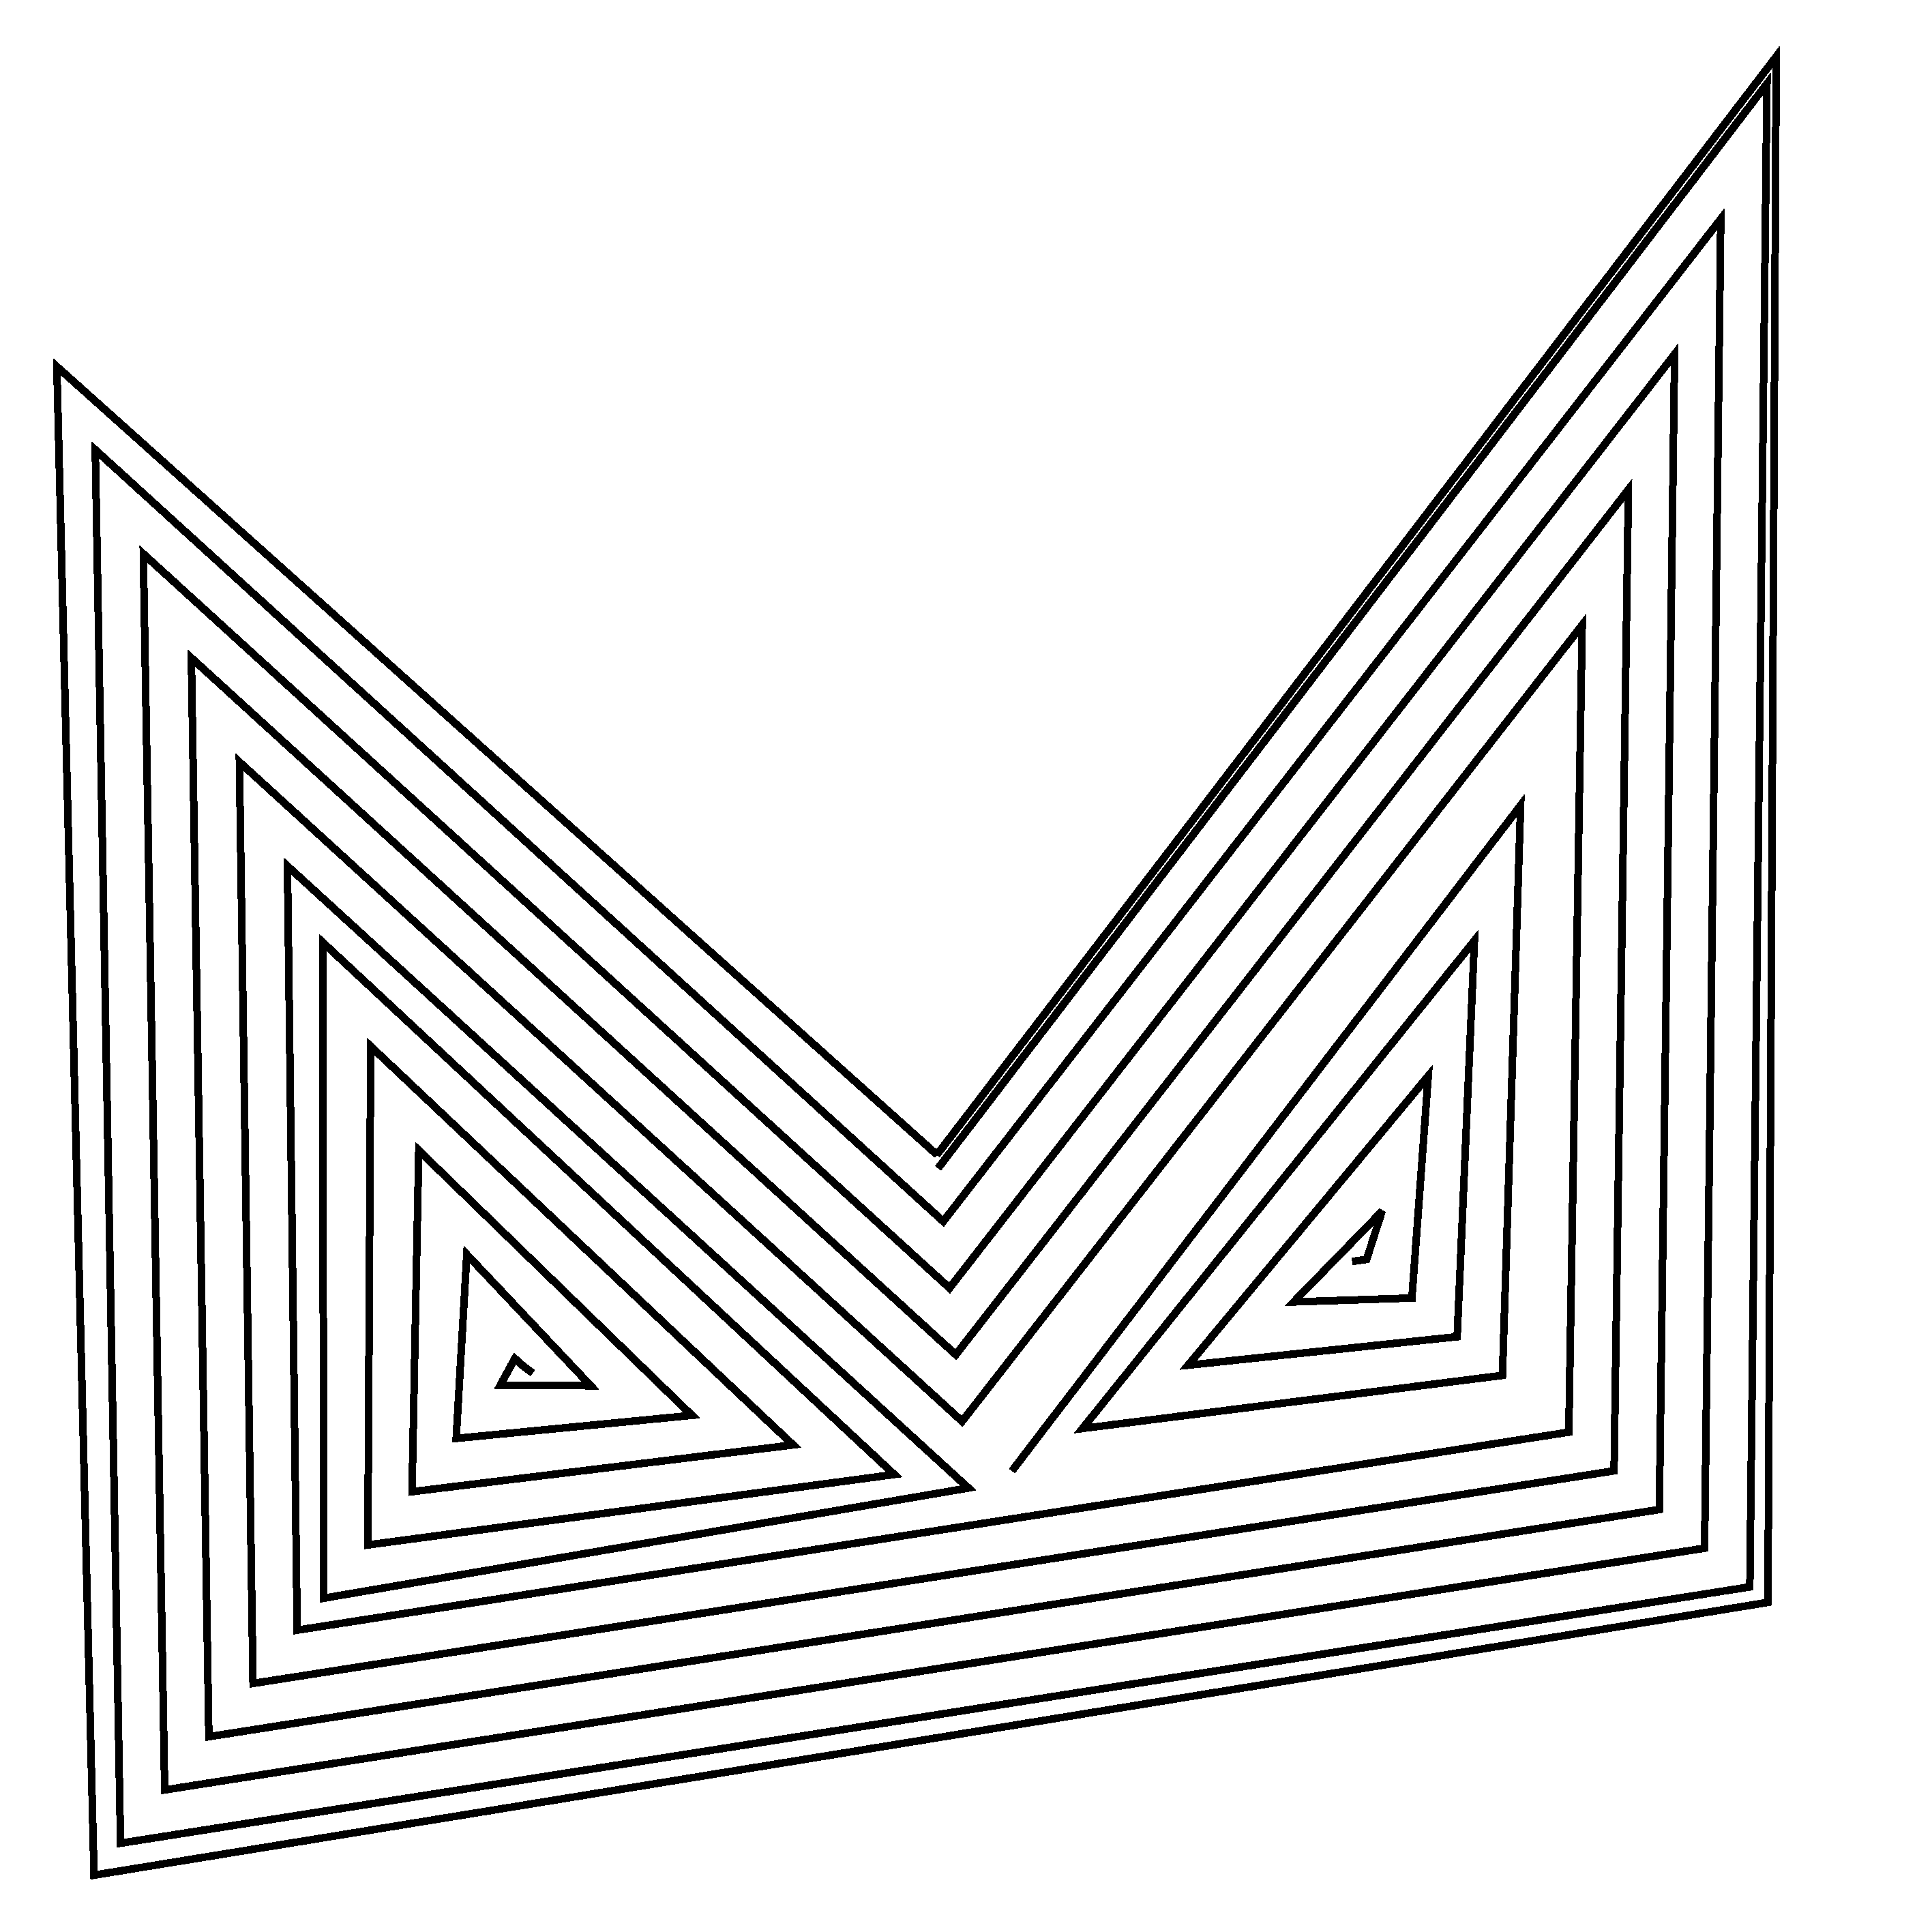
\includegraphics[width=0.6\textwidth]{images/algorithms/spiral_fill/spiral_real.pdf}
\caption{Generated spiral} \label{fig:gen_spiral}
\end{figure}

\clearpage

\subsection{Zig Zag Filling}

This fill method is quite straightforward: the polygon is filled by a number of lines that are parallel to each other and clipped at the polygon edges. The direction of the lines can be freely chosen.

To place the lines, the starting point is determined. If the chosen direction for the fill lines is inclined by more than 45°, the leftmost vertex is used as starting point, otherwise if the inclination is smaller, the bottommost vertex is selected.

Beginning from the starting point, a line in the specified direction is placed and the polygon edges are tested for intersection. If two intersections on the polygon edge for a given line are found, a line segment with those two intersection points is added to the resulting trajectory. The starting point of the line is translated by the specified rake width constant in the direction normal to the chosen direction and the process is repeated. In the case that no two intersections are found any more, the algorithm stops.

This method works very well for convex polygons, but is not applicable for non-convex polygons, since a non convex polygon can have more than two intersections for any given line. Therefore it requires the polygon to be decomposed into convex parts. It was decided to use the optimal convex partitioning with the algorithm by Greene \cite{greene1983decomposition}. The decomposed parts have vertices that coincide with the original vertices. Since it is an optimal convex partitioning algorithm, the number of created convex polygons is minimal (therefore the size of each decomposed part is maximized). Having larger decomposed parts is positive for the trajectory, because fewer turns in general reduce the drawing time and make for a more consistent look.

Additionally, the created segments (or the convex polygon) are offseted by a certain margin inwards to make way for the turns and reduce the amount of drawing that extends to the outside. As last step, each segment is driven with the rake lowered and the complete polygon is also traversed.

Because the Zig Zag filling can be thought of as one continuous line, all generated lines are connected with an \textit{enforced connection} (which is explained later) to reduce the amount of free connection points that the Traveling Salesman algorithm has to examine.
\begin{figure}
\centering
\begin{subfigure}[b]{0.6\textwidth}
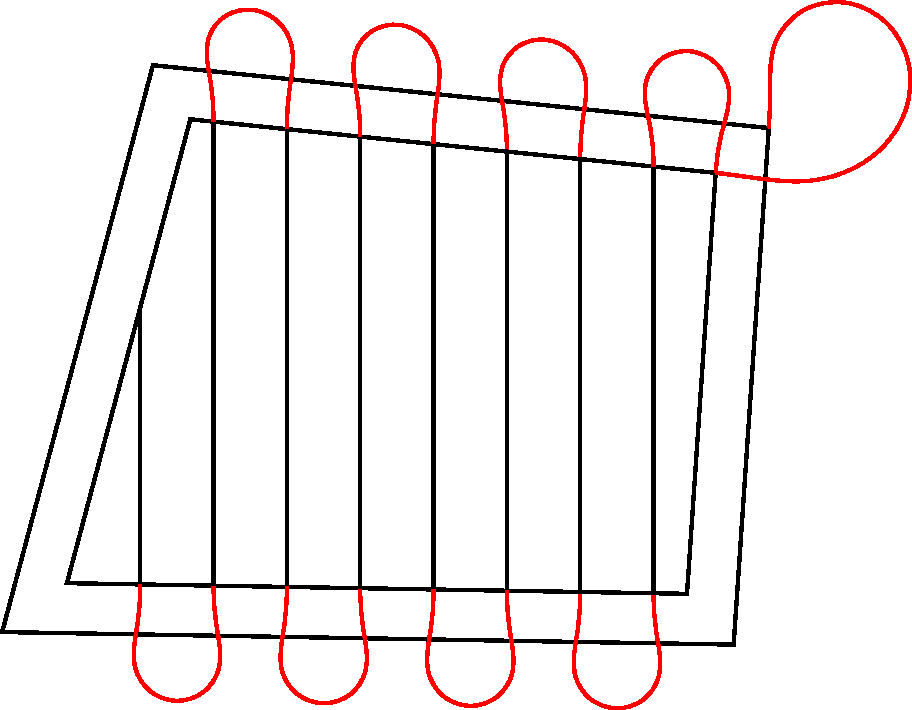
\includegraphics[width=\textwidth]{images/path_planning/zigzag_1.pdf}
\end{subfigure}
\par\bigskip
\begin{subfigure}[b]{0.9\textwidth}
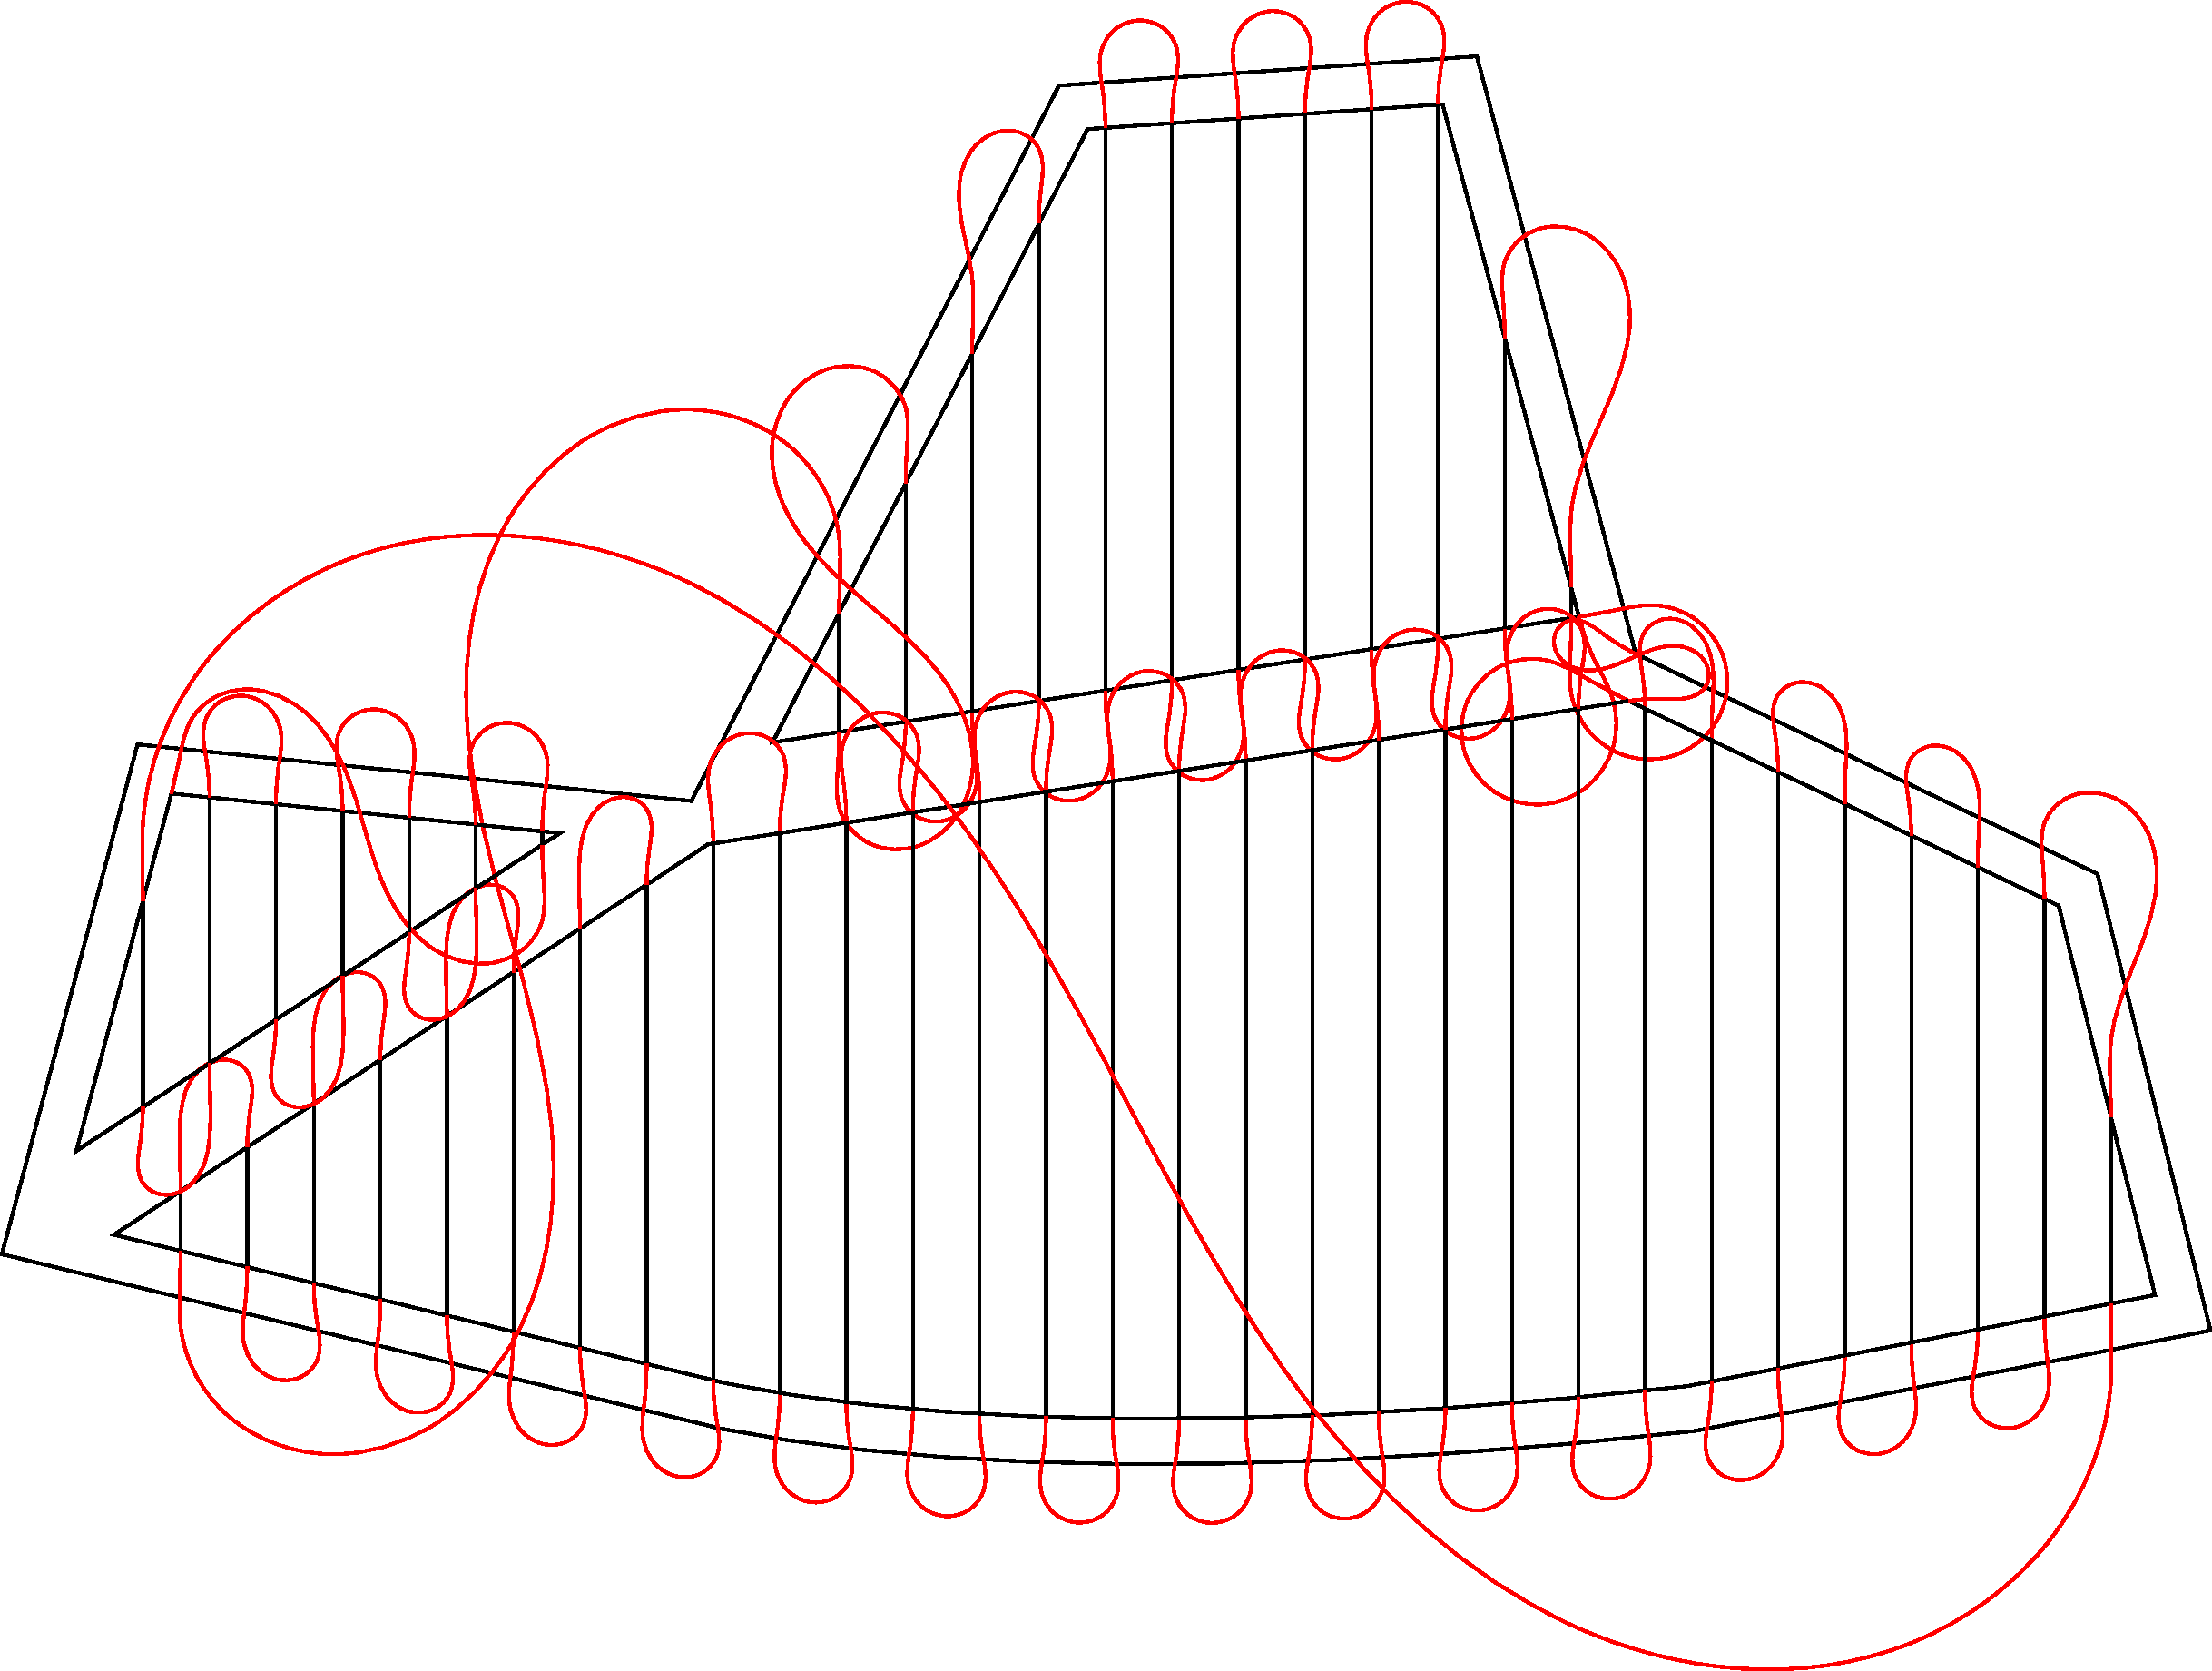
\includegraphics[width=\textwidth]{images/path_planning/zigzag_2.pdf}
\end{subfigure}
\caption{Zig Zag filling of two shapes. The first shape is convex, the second concave. The second shape is partitioned into convex elements using the optimal convex partitioning, which are separately filled with the Zig Zag fill.}
\end{figure}

\begin{figure}
\centering
\begin{subfigure}[b]{0.8\textwidth}
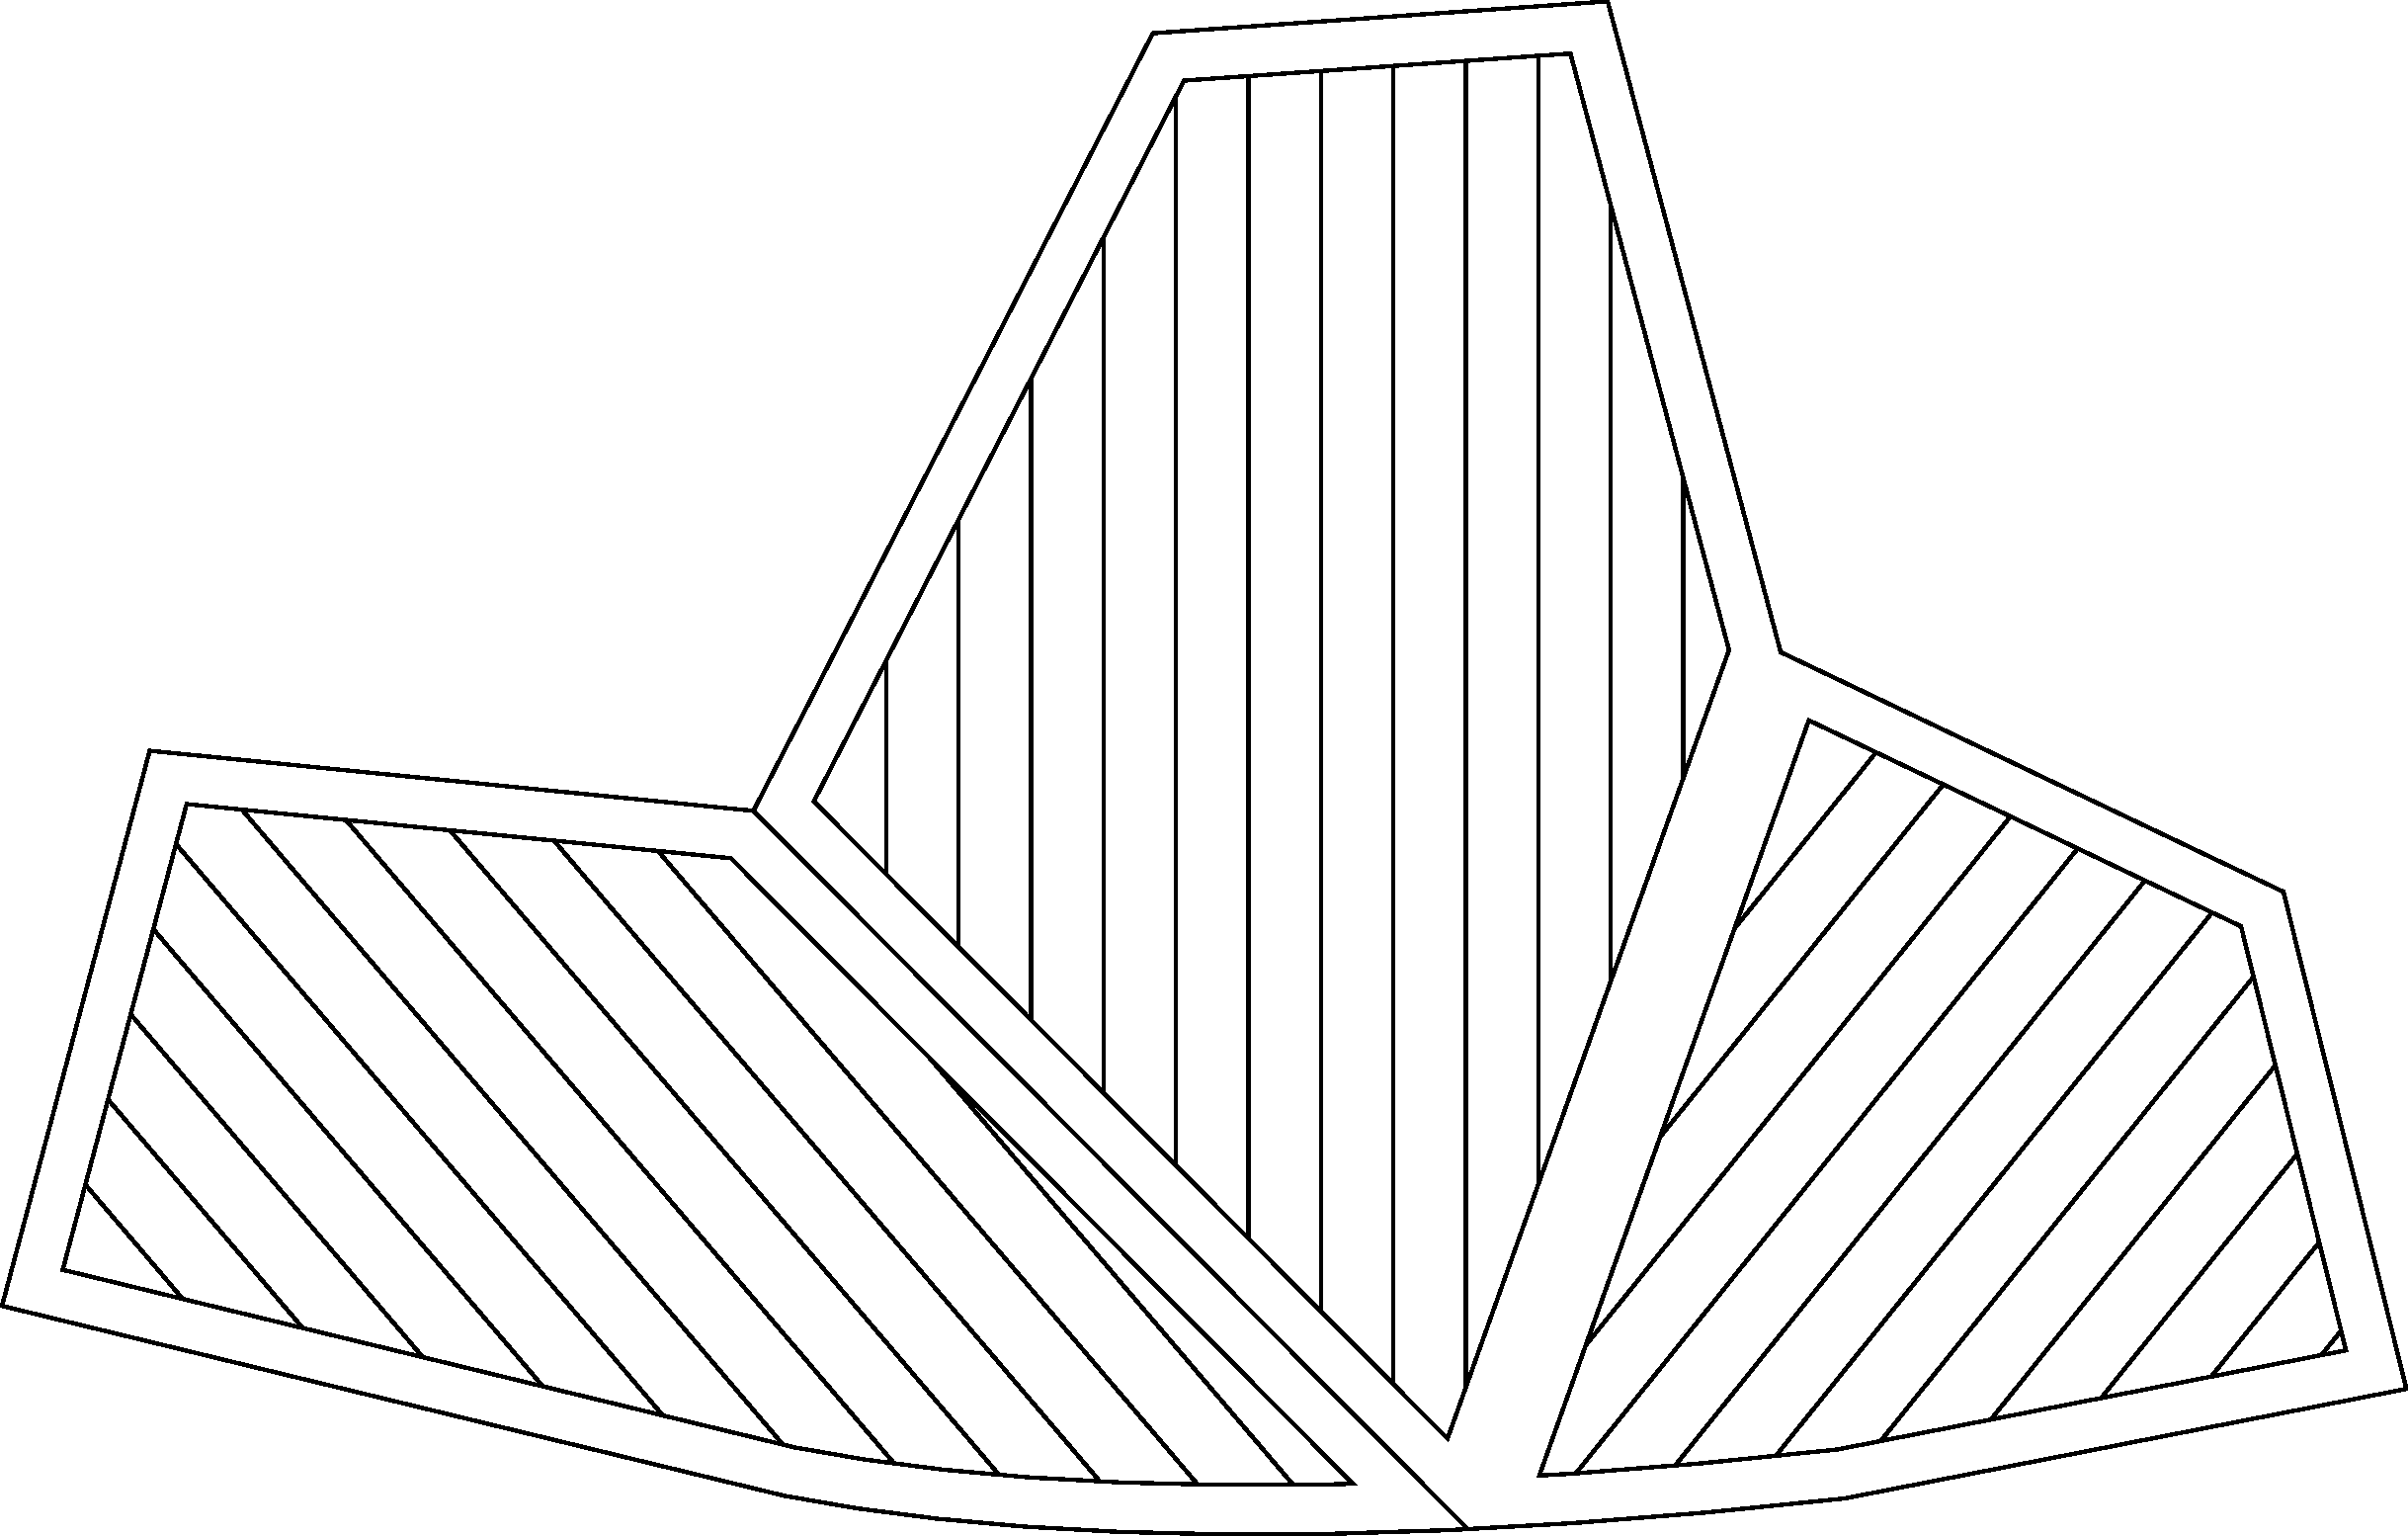
\includegraphics[width=\textwidth]{images/path_planning/zigzag_user_segment_and_fill.pdf}
\end{subfigure}
\caption{Users can choose an arbitrary segmentation and Zig Zag direction in the user interface}
\end{figure}

\section{Path Generation}
As already mentioned, to finally create a drawing all elements have to be connected by support trajectories that are not part of the drawing (where the robot drives with the rake lifted). The supporting paths should have two properties: the total distance of all support paths should be as small as possible and the curvature of the connections should be limited.

As previously defined, a drawing consists of the three different element types: lines, polygons and filled polygons. Lines and polygons differ in the way they can be connected, as illustrated in \autoref{fig:connect}. A line has two free connection points and is traversed from one end to the other. A polygon however can be entered at any vertex, but can only be exited at the same vertex so that it is closed. Filled polygons work the same as the regular polygon in that sense, since the spiral and the zig zag filling create a polyline which is inserted into the polygon.

\begin{figure}
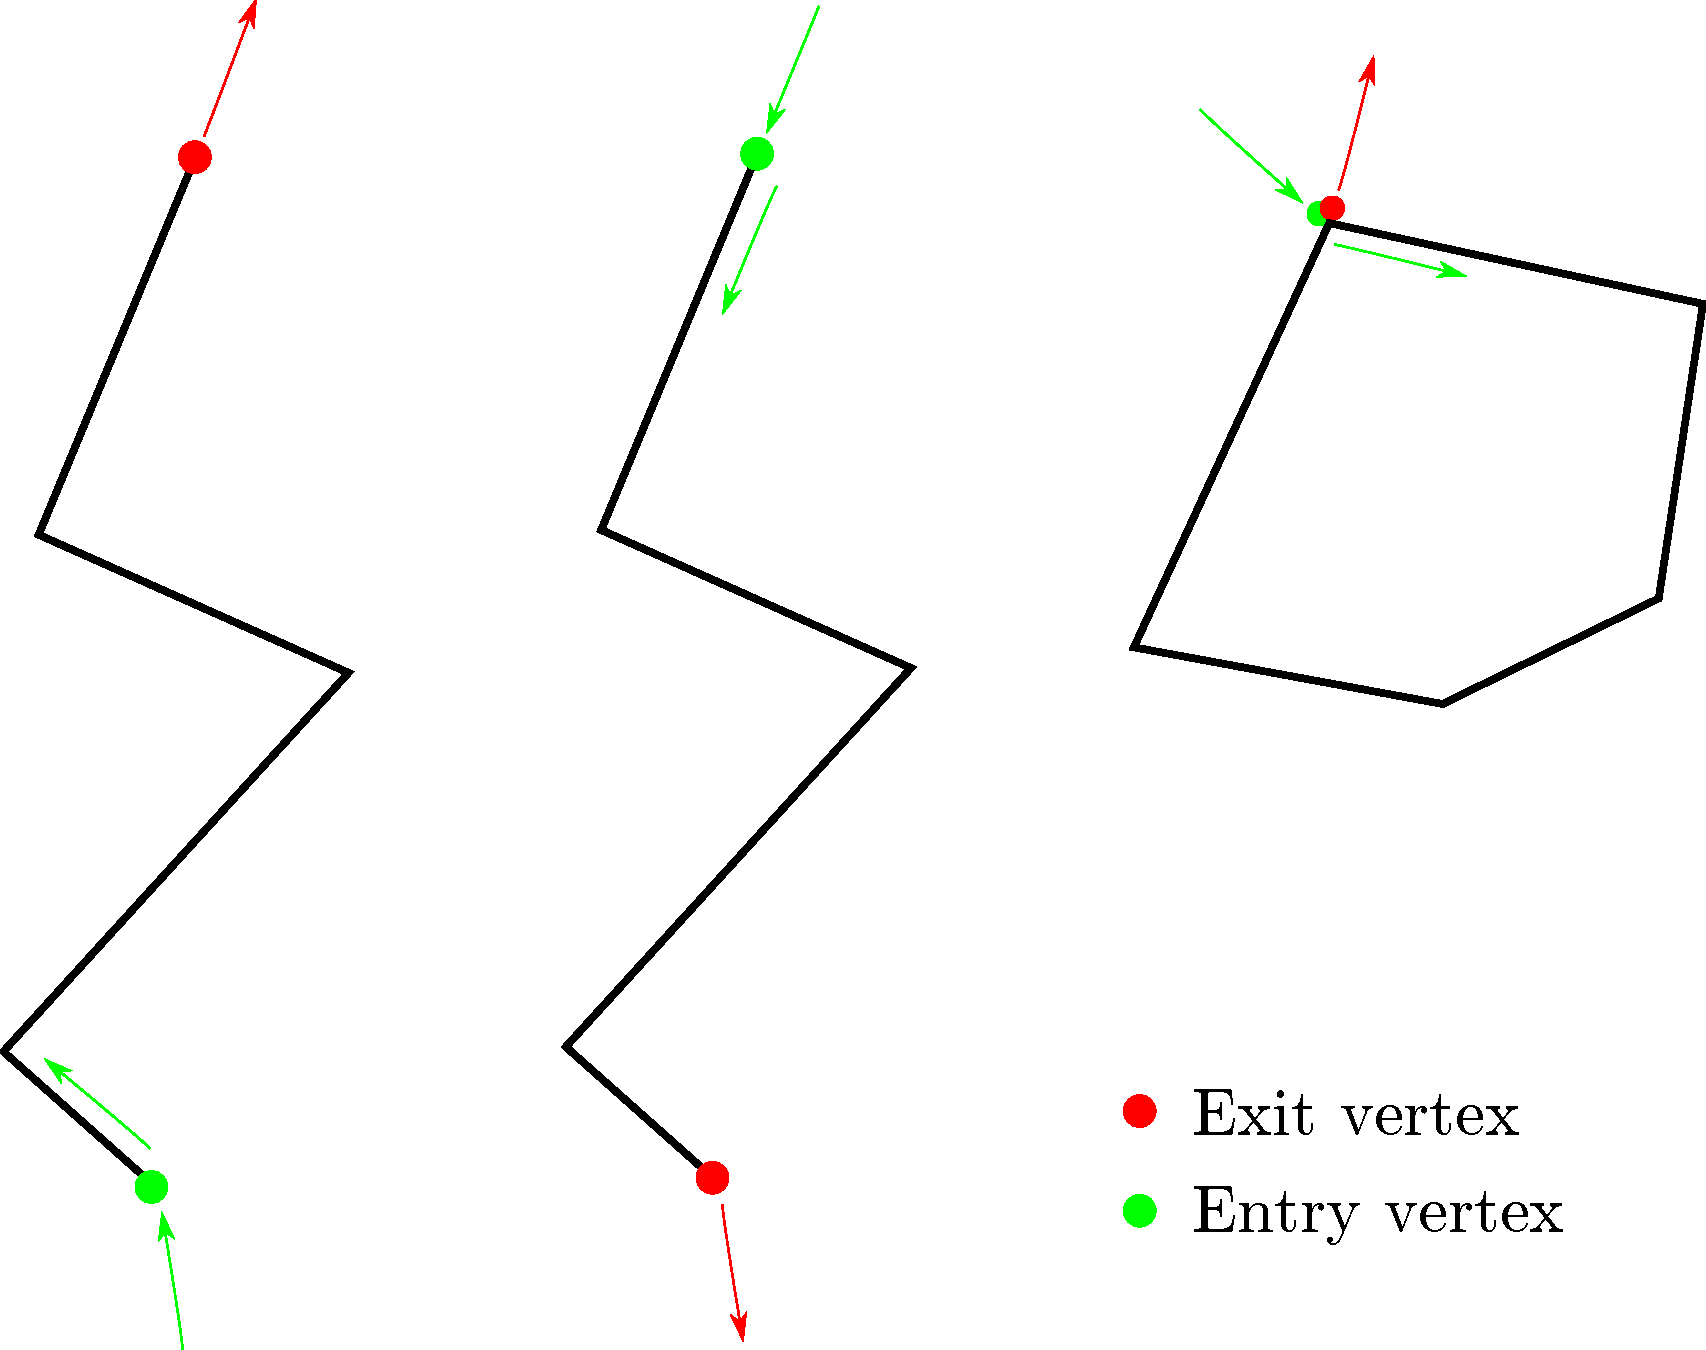
\includegraphics[width=0.8\textwidth]{images/path_planning/traversal.pdf}
\caption{Possible entry- and exit vertices and direction of traversal for polylines and polygons. Note that the polygon could also be traversed in clockwise direction.}\label{fig:connect}
\end{figure}

\subsection{Traveling Salesman Problem}

The task of connecting the drawing elements is similar to that of a Travelling Salesman Problem.
The \textit{Travelling Salesman Problem} (TSP) is the problem of finding the minimum-weight Hamiltonian Circuit in a weighted graph. A weighted graph is a graph where every edge between two vertices has a certain weight associated. The Hamiltonian Circuit is defined as a tour through the graph that travels to every vertex exactly once forms a cycle. It is called travelling salesman problem because in the historical context the vertices were cities, the weights Euclidean distances and the salesman, seeking to minimize the distance travelled to do a round-trip through all the cities in a given tour, would seek to obtain a solution for this problem. However, one of the properties of the TSP that make this problem difficult to solve is that it is \textit{Non-deterministic Polynomial-time hard} (NP-hard) which means that, although the non-existence has not yet been proven, there is as of now no polynomial-time solution. If no heuristic is used, the amount of solutions that have to be searched in order to test all available possibilities is \enquote{$n!$}.

The weights of the problem are usually defined in a distance matrix  $D^{n \times n}$ matrix, where $n$ is the number of vertices in the graph and the elements in the matrix are given by $d_{ij}$.

The following properties for a general Travelling Salesman Problem are defined:

\begin{description}
\item[Symmetric] A TSP is symmetric if all distances between every node pair are symmetric (equal) in both directions ($d_{ij} = d_{ji} ~ \forall ~ i, j \mbox{ , } D^\intercal = D$).
\item[Metric] In a metric TSP, all distances conform to the triangle inequality $d_{xy} \leq d_{xz} + d_{zy} $ which is, for example, true if the distances are calculated using the Euclidean distance formula between two points: $d_{ij} = \sqrt{(x_i -x_j)^2 + (y_i - y_j)^2}$. Or for the so called Manhattan distance which is defined as ${d_{ij}^M} = |x_i-x_j| + |y_i - y_j|$.
\item[Asymmetric] If $d_{ij} \neq d_{ji}$ for at least one distance pair, then the TSP is asymmetric. The triangle inequality is not guaranteed to be fulfilled any more.
\end{description}

The easiest heuristic to the TSP is the nearest neighbour search. From a given starting point the nearest and unvisited vertex is searched and connected. This is done until no more unvisited elements exist. Positive about the nearest neighbour approach is that the complexity is only growing linear to the search size. However, the obtained solutions are often of unsatisfying quality.

Another standard heuristic is the branch and bound method. It works by splitting the set of possible solutions into two sets and calculating an upper and lower bound for both sets. If the upper bound of the first set is lower than the lower bound of the second, the second is discarded (and vice versa). During the course of this thesis a variant of the depth-first branch and bound search was implemented. First, the graph is traversed until a tour is completed. Afterwards, another tour is recursively started. As soon as the travelled distance of the entire tour in the new branch gets higher than the current minimum tour, the branch is discarded. 
While this already reduces the search space, the effect becomes relatively small on larger problems (e.g. the first 6 out of 15 nodes might only seldom span a tour where the distance is higher than the current minimum, and it gets only worse). Only the basic version of the heuristic was implemented.

%The implementation has not been very mature, and it actually produces an optimal tour in the current implementation, which is not necessarily desired in a heuristic, that should sacrifice quality for speed. With more level-wise bounds it could have been further improved. 

While the branch-and-bound implementation could have been optimized by a good margin, it became clear that for a drawing of reasonable size a state-of-the-art implementation had to be found. Currently there are, among others, two well-known state of the art implementations for the TSP\footnote{according to \url{http://www.adaptivebox.net/CILib/code/tspcodes_link.html}}: Concorde\footnote{\url{http://www.math.uwaterloo.ca/tsp/concorde.html}} and the Improved Lin-Kernighan Heuristic of Helsgaun (LKH)\cite{helsgaun2000effective}\cite{kernighan1970efficient}. The Concorde solver is one of the best currently available solvers which produce an exact solution\cite{hornik2007tsp}. However, it only works with symmetric distance matrices. While it is possible to transform a general non-Euclidean asymmetric problem into a symmetric one, the resulting matrix is bigger (in the case of \cite{kumar1996asymmetric} the transformed distance matrix is of size $2n \times 2n$), which will increase the computation time. Furthermore, an exact solution is not needed. Contrary to the Concorde solver, the Improved LKH of Helsgaun is able to directly work with asymmetric distance matrices, which makes it an ideal candidate for the purpose of this thesis. Furthermore, it is using a heuristic which is not guaranteed to obtain optimal solutions, but optimal solutions are arguably not needed for the case of a sand drawing.

The Lin-Kernighan heuristic is a local search optimization algorithm that works by using 2--opt and 3--opt moves. For a 2--opt move, 2 connections between 4 vertices are cut and the only other possible connection is checked (there is only one other possible connection because otherwise two closed tours would result). If the resulting tour is shorter, it is picked as new basis tour. Repeating this step generates a more optimal solution each time.

An extension of the 2--opt move is the 3--opt move, where connections between 6 vertices (3 connections) are removed and all new connection possibilities are evaluated. The Lin-Kernighan algorithm extends this even further and works with $\lambda\text{--opt}$ moves. This generally degrades the runtime to $\mathcal{O}(n^\lambda)$. Therefore the Lin-Kernhighan algorithm uses variable $\lambda\text{-opt}$ moves: starting at $\lambda=2$ at each step is evaluated if $\lambda$ should be increased by one or not through applying a series of tests. At a stopping condition this process ends.

The author, Keld Helsgaun, also demonstrates how the specific LKH implementation is suited to solve the equality generalized\citep{helsgaun2013equality} as well as the clustered TSP\cite{helsgaun2014solving}. A combination of both cases is used in this thesis to find a high quality tour through the drawing of.

The LKH solver uses the \textit{TSPLIB}\footnote{\url{http://www.iwr.uni-heidelberg.de/groups/comopt/software/TSPLIB95/}} file format as interface to read and write the problems. The TSPLIB is a benchmark collection of various traveling salesman problems, where some of them have known optimal solutions.

%The final solution to the minimum connection problem was to use a state of the art TSP solver\cite{helsgaun2000effective}, which employs the Lin-Kernhighan-Heuristic\cite{kernighan1970efficient} (LKH) to approximately solve the Traveling Salesman Problem. It is, unlike many other TSP solver implementations that require the triangle inequality to hold, also well suited to solve assymetric problems.
% general definition
% all three methods we tried, including LKH
\subsection{Adaptation of Traveling Salesman Problem for the Algorithm}

To find a suited tour with the generic LKH solver, the correct weights for the distance matrix have to be specified. The term \enquote{outgoing} is used for all weights from one specific vertex to all other vertices and \enquote{ingoing} for the weights from all vertices of the graph to one vertex. This happens in the following steps:

\begin{itemize}
\item On polylines, all vertices that are not the first or last node are removed, since they can never be accessed without entering at either the first or last node 
\item Polygons can be entered at any node. However, once entered, the polygon cannot be exited at any location but must be traversed completely. To enforce this, the weights on the polygon edges are set to be zero for the next vertex in clockwise direction and infinity for all other nodes of the polygon.
\item Every node is only visited once. This leads to problems in polygons, where the tour should be closed. There are two possible solutions: double cities or weight shifting. With the double cities approach (illustrated in \autoref{fig:doublecities}), each vertex on the polygon is added two times to the distance matrix: one with Euclidean distances as ingoing weights and all outgoing weights set to $\infty$ and the second with Euclidean distances as outgoing weights and ingoing weights set to $\infty$. The weights between all cities on the polygon are set to zero in one direction, i.e., clockwise (also between the double cities). Therefore the exit city has to be positioned \textit{behind} the entry city, so that it is the last visited city by the algorithm which is forced to close the circuit around the polygon. Since the double cities approach is doubling the number of cities it is clearly the less optimal approach. Because it is known that entering at node $n$ will result in the visitor ending up at node $n-1$ if all edges are zero, using the weight shifting method, the outgoing weights of the polygon at node $n$ are shifted to node $n-1$. Thereby, the element-wise symmetry is restored and a optimal solution can be found with a generic TSP solver. In a post processing step, the polygon is closed again.
\item All other edge weights are the Euclidean distances between each vertex pair.
\item A regular TSP tour is closed. This implies that a regular tour has a tendency to go back to the starting point after diverging into another direction at the start of the tour. The solution that was found is to enforce a defined starting point with special properties to be inserted. The outgoing weights of the start point are either euclidean distances or defined to be set to the same value to every node in the graph. If they are euclidean, it is very likely that the first visited line is the nearest neighbour. If the outgoing weights are all defined to be a constant value the LKH can find the best suited first tour point on its own because the starting point will not induce any preference for any of the nodes.
With the same reasoning, the weights pointing back to the starting point are chosen to be equal for all nodes. Thus, the TSP will never optimize towards travelling back to the starting point.
\end{itemize}

How the weights are aquired is also illustrated in \autoref{fig:illdistweights}. The distance matrix of a simple drawing is shown in \autoref{simple_tsp_fig}.

\begin{figure}
\centering
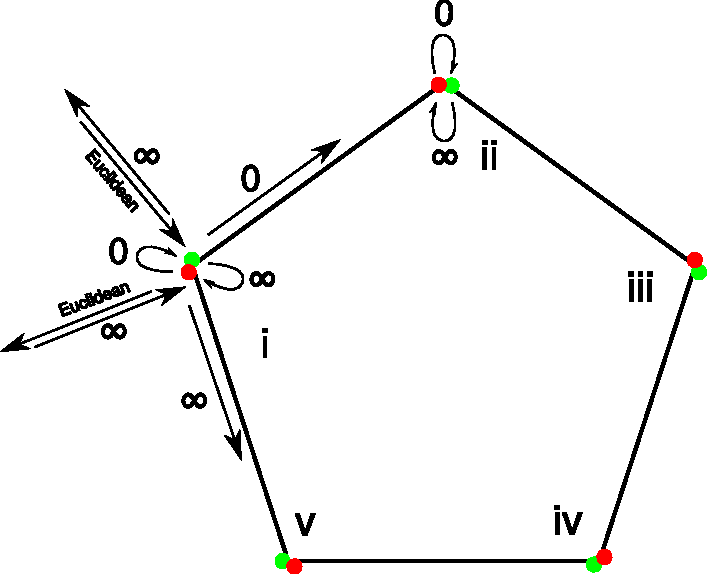
\includegraphics[width=0.8\textwidth]{images/path_planning/double_cities.pdf}
\caption{Double cities approach to solve the TSP on a polygon.}\label{fig:doublecities}
\end{figure}

\paragraph{Reprojecting the Tour} The output of the LKH algorithm is a text file with ordered \textit{tour indices} (shown in \autoref{tour_output_eq}). The text file is read back in the main program and evaluated. Since the LKH algorihtm is not aware of the structure of the problem at hand, the indices have to be \enquote{projected} to the drawing elments. The tour indices correspond to the matrix indices and the ordering is that of the shortest found tour through the elements, vertex by vertex.
To connect all elements in the way the tour was found, first the tour starting point is searched among the tour indices (the tour starting point index is always \enquote{1}).

All other indices have to be saved beforehand and need to be reapplied now: The tour index corresponds to a vertex on a given element. The elements are now connected in the order they appear in the found tour. For the connection only the first tour index on each element is relevant, because the exit point of the element is trivially known for each type of element when the entry point is given.
 
\paragraph{Enforcing Connections} If the found solution is not sufficient or satisfying, the user might want to alter the tour. This works through the enforcement of connections between two points on the elements. If two elements have an enforced connection, they can be represented by a single line with entry and exit point and an unknown traversal direction. This is due to the fact that if one point on an element is connected, there is a trivially known other point that is the last available connection point. For example, if a polygon has an enforced connection at vertex $v_i$, it is known that $v_i$ will also be either start- or endpoint for the connected elements because the polygon loop has to be closed. Similarly, if the first or last point of a polyline has an enforced connection the other is the remaining free connection point that can be used to connect to other elements. Thus, instead of the single elements, the start and endpoint of said \enquote{imaginary} polyline are added to the distance matrix and the tour is completed during the post processing. An element with two enforced connections is completely ignored in the distance matrix, since it has no free connection points.

\paragraph{Containment Properties}

A polygon can enclose other elements, such as a polygon or a set of lines. Generally, to avoid crossing too many lines, it is undesired to enter this enclosing polygon twice. Therefore the weights of the polygon vertices towards the inner elements are set to infinity. Thus the tour will always start on the inside and continue to travel further outside.

\begin{figure}
\centering
\begin{subfigure}[b]{0.45\textwidth}
\centering
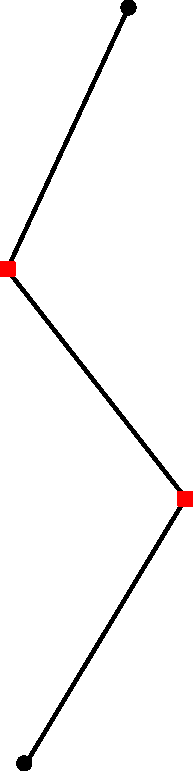
\includegraphics[height=6cm]{images/path_planning/tsp_polyline.pdf}
\caption{A polyline. The red squares (inner vertices) will be removed in the distance matrix as they cannot be reached from the \enquote{outside}.}
\end{subfigure}
~
\begin{subfigure}[b]{0.45\textwidth}
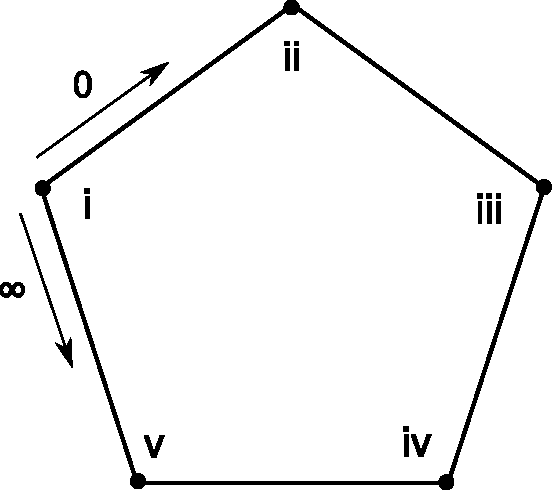
\includegraphics[width=1\textwidth]{images/path_planning/tsp_polygon.pdf}
\caption{A polygon with the traversal direction on the polygon itself: Only the clockwise direction is allowed (arbitrarily chosen).}
\end{subfigure}

\par\bigskip

\begin{subfigure}[t]{0.45\textwidth}
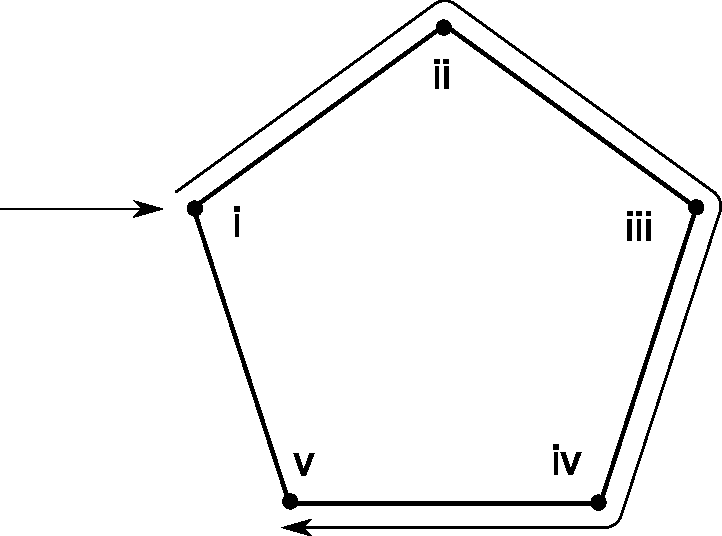
\includegraphics[width=1\textwidth]{images/path_planning/tsp_polygon_2.pdf}
\caption{Entering the polygon at node (i) it is known that the exit vertex must be (v), because no vertex is visited twice and all intermediate edges have a weight of zero.}
\end{subfigure}
~
\begin{subfigure}[t]{0.45\textwidth}
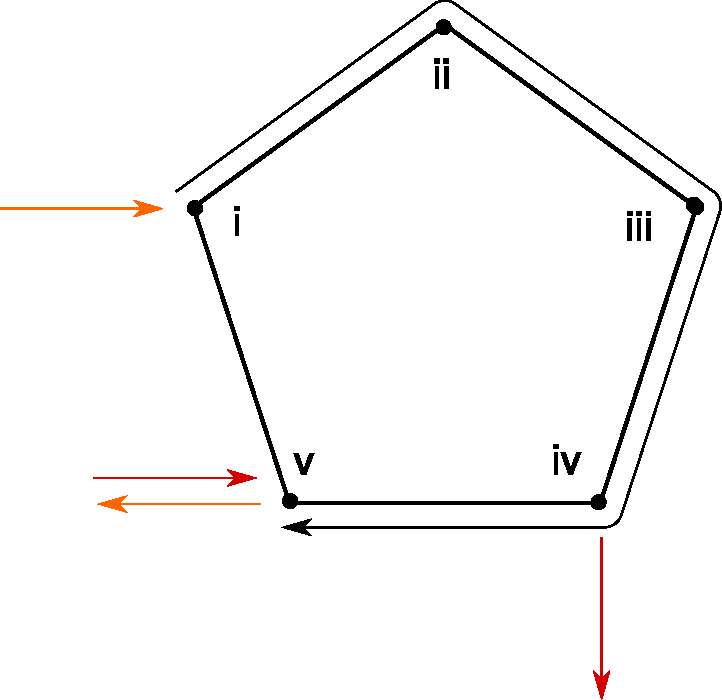
\includegraphics[width=1\textwidth]{images/path_planning/tsp_polygon_3.pdf}
\caption{Because the exit node is known, the outgoing weights from node (i) are shifted to node (v). Since the polygon can be entered from any vertex, the same happens to all vertices in the polygon.}
\end{subfigure}
\caption{Illustrating how weights for the distance matrix are determined}\label{fig:illdistweights}
\end{figure}


\begin{figure}[h]
\centering
\begin{subfigure}[b]{1\textwidth}
\centering
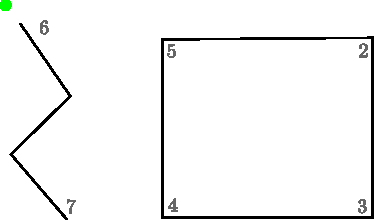
\includegraphics[width=0.6\textwidth]{images/path_planning/simple_tsp_figure.pdf}
\caption{Simple TSP figure: tour startpoint in green, and two elements. Note that the \enquote{inner} vertices of the polyline are removed in the matrix. Gray numbers indicate corresponding matrix indices.}
\end{subfigure}

\par \bigskip

\begin{subfigure}[b]{1\textwidth}
\[
D=\left(
\begin{array}{ccccccc}
- & 1812 & 2097 & 1328 & 806 & 156 & 1127 \\
1 & - & 0 & \infty & \infty & 1959 & 1489 \\
1 & \infty & - & 0 & \infty & 1173 & 467 \\
1 & \infty & \infty & - & 0 & 698 & 993 \\
1 & 0 & \infty & \infty & - & 1717 & 1732 \\
1 & 1717 & 1959 & 1173 & 698 & - & 0 \\
1 & 1732 & 1489 & 467 & 993 & 0 & - \\
\end{array}
\right)
\]
\caption{The corresponding matrix: First row and column are values of the tour start point. Thereafter, the distances of the polygon follow (note how the zeros are shifting and the shifted symmetry of the rightmost columns and bottom rows). The last two entries correspond with the polyline (where the two inner vertices are removed).}
\end{subfigure}
\par \bigskip
\begin{subfigure}[b]{1\textwidth}
\[
\left\{ 1, 6, 7, 4, 5, 2, 3, -1 \right\}
\]
\captionsetup{singlelinecheck=off}

\caption[Tour indices]{The indices of the shortest tour through the drawing, as returned by the LKH application. 
\begin{itemize}
\item Index 1: tour starting point
\item Indices 6 \& 7: points on the polyline
\item Indices 4, 5 2, 3: points on the polygon
\item Index -1: indicates return to start (end of tour).
\end{itemize}}\label{tour_output_eq}
\end{subfigure}
\caption{Drawing, TSP distance matrix and final tour for a simple drawing}\label{simple_tsp_fig}
\end{figure}

\clearpage
\section{Smooth Line Connections}

While not required by the robot kinematics of the BeachBot (which can turn on the spot), generating smooth connections 
makes the developed algorithms generalizable for four-wheeled vehicles.
It is also necessary to constrain the curvature for the path converter that translates the generated rake path into a robot path that is drivable by the bot. If the curvature at a given point of the connection is too high, it is not possible for the path converter to find a converging solution which makes tedious manual work needed to adjust the curvature of the connections until the converter is able to find a solution. The rounded connections would also create a nice visual effect for spectators.

Ideally a way would have to be found that limits the curvature of the connection path.

Curvature is defined as the inverse of the radius of the circle that the tangent produces at any given point in the curve. For a two dimensional curve, the curvature $\kappa$ is defined as 
$$\kappa = \frac{|x'y''-y'x''|}{(x'^2+y'^2)^{3/2}}$$


\subsubsection{Beziér Splines}

A first approach to generate more curved connections was to use Beziér splines.
The start- and endpoint of the beziér spline is trivially found as the start- and endpoint of the connection. As first solution, we used beziér splines of 3rd order. Beziér splines of 3rd order only yield 2 control points, which can, by moving them along the desired tangent, easily be used to create a connection that is smooth in the start and endpoint. However, the curvature for the complete curve can not be set because the two control points offer to few degrees of freedom. A beziér curve of 5th degree (quintic) has enough DOF to constrain the connection in terms of curvature.

The quintic Beziér curve consists of 6 control points $P_0 ... P_5$ that define the shape of the curve. $P_0$ and $P_5$ are trivially chosen because they coincide with the start- respectively the endpoint of the curves that should be connected. $P_1$ and $P_4$ are also easy to choose as they have to lie on the tangents of the curves that should be connected. $P_2$ and $P_3$ on the other hand are more difficult to obtain. Even after an extensive search through available literature it remained unclear if an analytical solution to this problem can be found or not, since the equation for curvature is getting quite complicated if expanded. In \cite{doi:10.1137/1.9781611971521.ch5} three approaches to generate beziér splines with monotone curvature are discussed. \cite{choi2010piecewise} uses piecewise 3rd degree bezier curves to create a curvature and corridor constrained trajectory.  [to be expanded]

\subsubsection{Spiro Splines}

Spiro splines, introduced by R. Levien \cite{levien2009spiral} are a different approach to designing fair curves, initially for the purpose of designing fonts. They have several properties which make them well-suited for the task at hand:

They offer 4 different control points to control the shape of the curve. In contrast to beziér curves, spiro spline control points are always passed by the generated curve, whereas the bezier curve only goes through the first and last control point. The 4 different control points, denoted by a single character, of spiro splines are:

\begin{itemize}
\item[\texttt{v}] Corner point
\item[\texttt{c}] A $G^2$ continous constraint. The curvature  on the left side is the same as on the right side ($\kappa_l = \kappa_r$).
\item[\texttt{o}] Similiar to \texttt{c}, a $G^4$ continous constraint. Not only $\kappa_l = \kappa_r$ is true, but also the first and second derivative of the curvature is constrained ($\kappa_l' = \kappa_r'$, $\kappa_l'' = \kappa_r''$).
\item[\texttt{[}] A straight-to-curved control point that acts like a tangent constraint in this case.
\item[\texttt{]}] A curved-to-straight control point that also acts like a tangent constraint here.
\end{itemize}

The author, Raph Levien, has licensed his implementation \footnote{libspiro: \url{http://www.levien.com/spiro/} } of spiro splines under the GPLv2, which makes it possible to be used by this thesis. The implementation is capable of being used for realtime editing. That guarantees that the curve generation would not be the bottleneck of the application in terms of time consumption. The output of the library is a set of Beziér curves which are easier to handle in regular graphics programs.

\paragraph{Heuristic for Setting the Control Points}

To find suitable locations for the spiro spline control points, a heuristic was used.

All connection constraints can be expressed by 5 variables: Connection length ($d$), tangents with angles $\alpha$ and $\beta$ and the curvature limit $\kappa$, as shown in \autoref{fig:connection_vars}. For the calculation of the control points, the difference between the two angles was defined as $\delta = \alpha - \beta$. It equals the angle between the two tangent vectors. 

Finding the first 4 points of the curve is straightforward: The first control point is a corner point at the endpoint of the first element. The second point is a straight-to-curve point, that is positioned an infinitesimally small distance in the direction of the tangent from the first point. This constrains the \enquote{outgoing} tangent. Vice versa, the same control points are set at the end of the curve, where the element that is connected with begins. Thus both tangent constrains are fullfilled. Because the spiros do not offer a direct way of setting the maximum and minimum curvatures, zero to two more control points have to be added. The curvature can be limited by positioning a $G^2$ control point at distance $2 * R$ from the start- and endpoint. This limits the curvature to the left and to the right to be the same. Since the highest curvature between the startpoint and the $G^2$ point would be a circular arc with radius $R$ this limits the curvature to $\kappa = 1/R$, as long as both $G^2$ points are keeping a distance of $2*R$ as well.

The heuristic differentiates 3 cases:

If the both tangent vectors $\alpha$ and $\beta$ have a similar direction and the circle that is described by them and $d$ has a radius that is in the range of $R < r < 2*R$ then no intermediate $G^2$ points are set because the connection will already be smooth and optimal.

Otherwise, the $G^2$ points are set by elongating the tangent vector to $2*R$ and rotating it by $0.5 * \alpha$. This is done to reduce the size of the resulting curve, which is demonstrated in .. Fig ...

As discussed, the two $G^2$ points, called $c_1$ and $c_2$ are closer than $2 * R$ to each other, the positions have to be recalculated. This happens by rotating the $c_1$ and $c_2$ points gradually in different direction until positions are found that conform to the distance constraint. By rotating both points about the same angle, a symmetry is kept.

If the distance $d$ is smaller than 

\begin{figure}

\usetikzlibrary{calc}

\definecolor{cb3b3b3}{RGB}{179,179,179}
\definecolor{ccccccc}{RGB}{204,204,204}
\definecolor{cffffff}{RGB}{255,255,255}

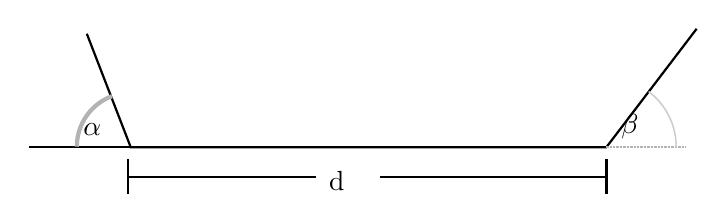
\begin{tikzpicture}[y=0.80pt,x=0.80pt,yscale=-1, inner sep=0pt, outer sep=0pt]
\centering
  \path[draw=black,line join=miter,line cap=butt,line width=0.800pt]
    (96.0814,121.3474) -- (115.9166,172.6195) -- (330.7355,172.6195) --
    (371.5287,119.1019);
  \path[draw=black,line join=miter,line cap=butt,line width=0.800pt]
    (115.9129,172.6241) -- (69.8665,172.6241);
  \path[draw=cb3b3b3,dash pattern=on 0.34pt off 0.17pt,line join=miter,line
    cap=butt,miter limit=4.00,dash phase=0.201pt,line width=0.800pt]
    (330.6888,172.6195) -- (366.5496,172.6195);
  \path[cm={{1.45393,0.0,0.0,1.45393,(-471.01666,-377.22731)}},draw=ccccccc,miter
    limit=4.00,line width=0.550pt] (564.5997,360.8878)arc(-52.961:0.593:21.466);
  \path[cm={{0.52395,0.0,0.0,0.52395,(41.81533,-25.47312)}},draw=cb3b3b3,miter
    limit=4.00,dash phase=0.960pt,line width=1.527pt]
    (94.9543,377.5908)arc(179.987:249.624:46.467);
  \path[fill=black,line width=0.800pt] (94.482018,167.26112) node[above right]
    (text4046) {$\alpha$};
  \path[fill=black] (337.53653,168.90082) node[above right] (text4046-2)
    {$\beta$};
  \path[draw=black,line join=miter,line cap=butt,line width=0.800pt]
    (114.8543,177.9195) -- (114.8543,193.7975);
  \path[draw=black,line join=miter,line cap=butt,line width=0.800pt]
    (114.8543,186.1205) -- (330.7957,186.1205);
  \path[draw=black,line join=miter,line cap=butt,line width=0.800pt]
    (330.7957,177.9195) -- (330.7957,193.7975);
  \path[fill=cffffff,line width=0.800pt,rounded corners=0.0000cm]
    (199.5575,177.5072) rectangle (228.2820,192.5707);
  \path[fill=black,line width=0.800pt] (205.50471,192.37236) node[above right]
    (text4081) {d};
\end{tikzpicture}
\caption{Variables for the connection between two elements}
\label{fig:connections_vars}
\end{figure}
